\documentclass[a4paper]{article}
\usepackage[margin=0mm]{geometry}
\usepackage{xcolor}
\usepackage{tikz}
\pagestyle{empty}
\begin{document}
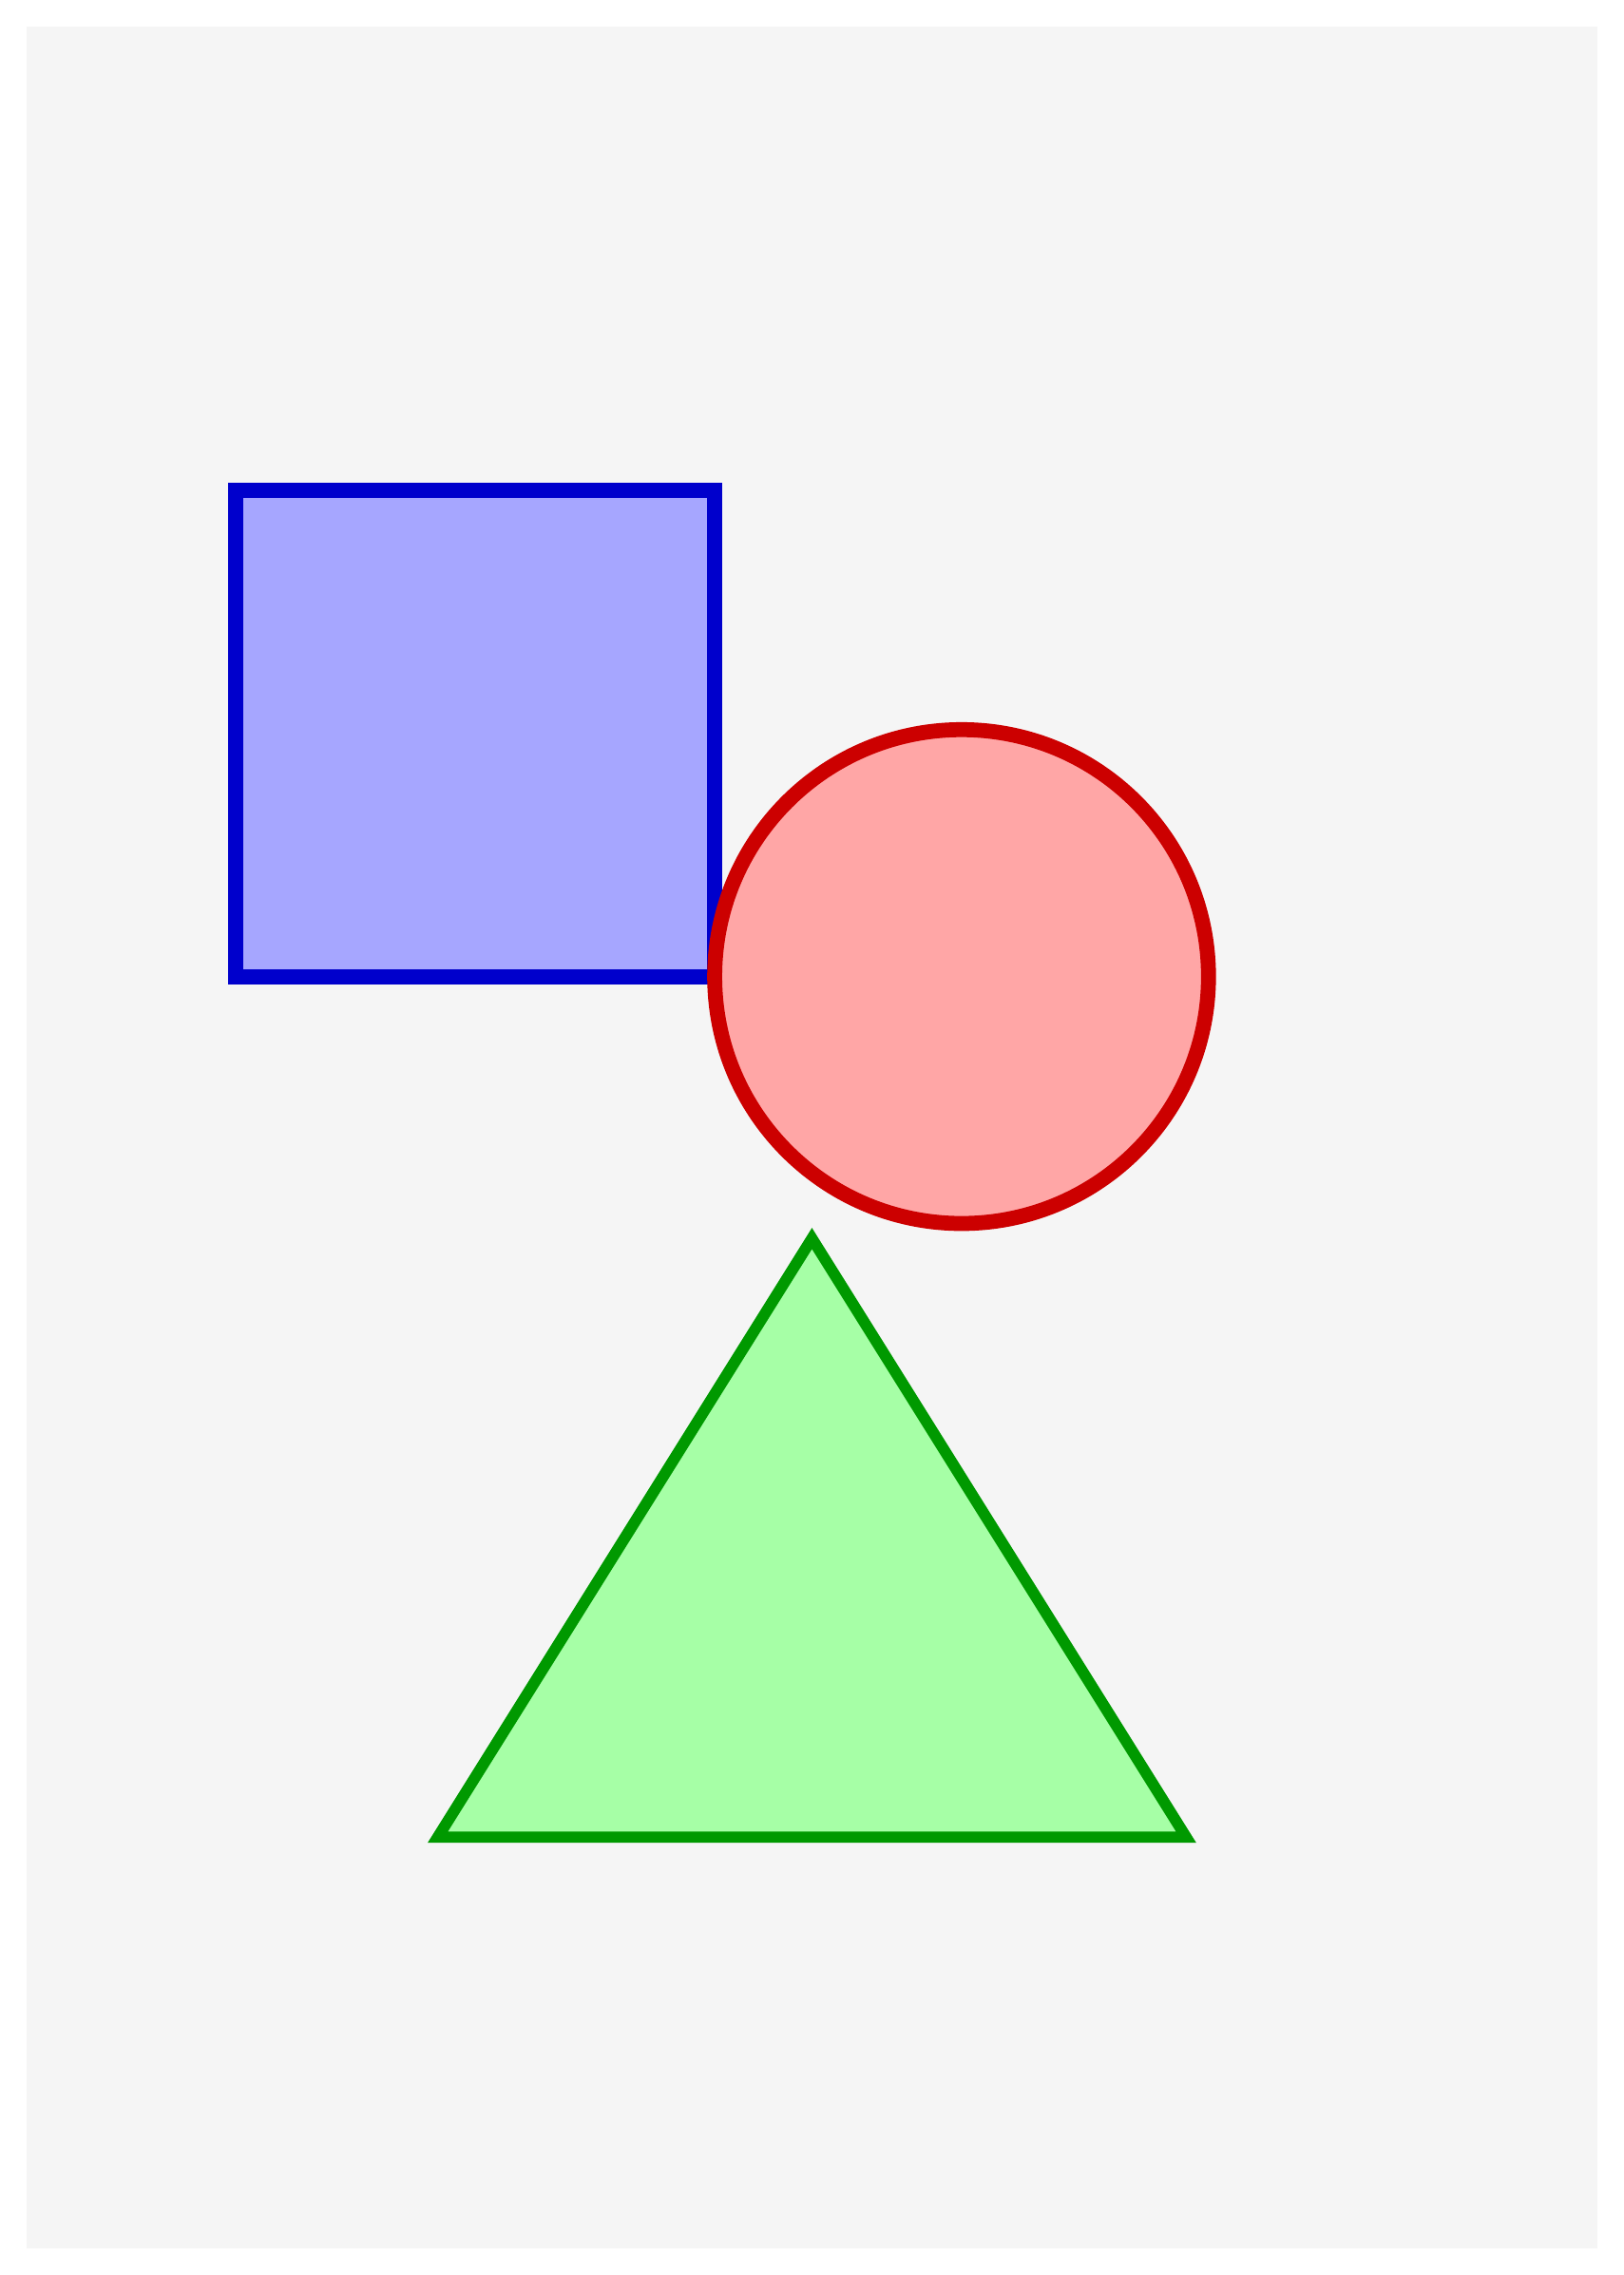
\begin{tikzpicture}[x=1mm,y=1mm]
\fill[gray!8] (0,0) rectangle (210,297);
\fill[blue!35] (28,170) rectangle (92,235);
\draw[blue!80!black,line width=2mm] (28,170) rectangle (92,235);
\fill[red!35] (125,170) circle (33);
\draw[red!80!black,line width=2mm] (125,170) circle (33);
\fill[green!35] (55,55) -- (105,135) -- (155,55) -- cycle;
\draw[green!60!black,line width=1.5mm] (55,55) -- (105,135) -- (155,55) -- cycle;
\end{tikzpicture}
\end{document}